\documentclass[modern]{aastex61}

% All the packages
%\usepackage[letterpaper]{geometry}
\usepackage{fontspec}
\usepackage{microtype}
\usepackage{url}
\usepackage{amsmath}
\usepackage{mathtools}
\usepackage{esint}
\usepackage{amssymb}
\usepackage{natbib}
\usepackage{multirow}
\usepackage{graphicx}
\usepackage{scalerel}
\usepackage{calc}
\usepackage{etoolbox}
\usepackage{marginnote}
\usepackage{nicefrac}
\usepackage{tabstackengine}
\usepackage{diagbox}
\usepackage[makeroom]{cancel}
\usepackage{mathdots}
\usepackage{bbm}
\usepackage{booktabs}
\usepackage{xspace}
\usepackage{upgreek}
\usepackage[T1]{fontenc} % https://tex.stackexchange.com/a/166791
\usepackage{textcomp}
\usepackage{ifxetex}
\ifxetex
\usepackage{fontspec}
\defaultfontfeatures{Extension = .otf}
\fi
\usepackage{fontawesome}
\usepackage{listings}
\usepackage{mathtools}
\stackMath

% Page breaks in long equations
%\allowdisplaybreaks

% Bibliography stuff
\bibliographystyle{aasjournal}

% Shorthand for this paper
\newcommand{\starry}{\textsf{starry}\xspace}
\newcommand{\batman}{\textsf{batman}\xspace}
\newcommand{\planetplanet}{\textsf{planetplanet}\xspace}
\newcommand{\Python}{\textsf{Python}\xspace}
\newcommand{\cpp}{\textsf{C}++\xspace}
\newcommand{\Mathematica}{\textsf{Mathematica}\xspace}

% editing
\newcommand{\todo}[1]{{\color{red}\textbf{TODO:} #1}}


% References to text content
\newcommand{\documentname}{\textsl{article}}
\newcommand{\figureref}[1]{\ref{fig:#1}}
\newcommand{\Figure}[1]{Figure~\figureref{#1}}
\newcommand{\figurelabel}[1]{\label{fig:#1}}
\renewcommand{\eqref}[1]{\ref{eq:#1}}
\newcommand{\Eq}[1]{Equation~(\eqref{#1})}
\newcommand{\eq}[1]{\Eq{#1}}
\newcommand{\eqalt}[1]{Equation~\eqref{#1}}
\newcommand{\eqlabel}[1]{\label{eq:#1}}

% Add code, proof, and animation hyperlinks
\definecolor{linkcolor}{rgb}{0.1216,0.4667,0.7059}
\newcommand{\codeicon}{{\color{linkcolor}\faFileCodeO}}
\newcommand{\prooficon}{{\color{linkcolor}\faPencilSquareO}}
\newcommand{\animicon}{{\color{linkcolor}\faPlayCircle}}
\input{gitlinks}

\newtagform{eqtag}[]{(}{)}
\newcommand{\currentlabel}{None}

% Define a proof environment
\newenvironment{proof}[1]{%
\ifstrempty{#1}{%
\renewtagform{eqtag}[]{\raisebox{-0.1em}{{\color{red}\faPencilSquareO}}\,(}{)}%
}{%
\renewtagform{eqtag}[]{\prooflink{#1}\,(}{)}%
}%
\usetagform{eqtag}%
\renewcommand{\currentlabel}{#1}
\align%
}{%
\endalign%
\renewtagform{eqtag}[]{(}{)}%
\usetagform{eqtag}%
\message{<<<\currentlabel: \theequation>>>}%
}

% Define a proof environment
\newenvironment{proof*}[1]{%
\ifstrempty{#1}{%
\renewtagform{eqtag}[]{\raisebox{-0.1em}{{\color{red}\faPencilSquareO}}\,(}{)}%
}{%
\renewtagform{eqtag}[]{\prooflink{#1}\,(}{)}%
}%
\usetagform{eqtag}%
\renewcommand{\currentlabel}{#1}
\equation%
}{%
\endequation%
\renewtagform{eqtag}[]{(}{)}%
\usetagform{eqtag}%
\message{<<<\currentlabel: \theequation>>>}
}

% Math stuff
%\newcommand{\ii}{\ensuremath{\mathbf{i}}}
\newcommand{\T}{\ensuremath{\mathrm{T}}}
\newcommand{\dd}{\ensuremath{ \mathrm{d}}}
\newcommand{\unit}[1]{{\ensuremath{\mathrm{#1}}}}
\newcommand{\bvec}[1]{{\ensuremath{\mathbf{#1}}}}
\newcommand{\avec}[1]{{\ensuremath{\vec{\mathbf{#1}}}}}
\newcommand{\x}{\ensuremath{\mbox{$x$}}}
\newcommand{\y}{\ensuremath{\mbox{$y$}}}
\newcommand{\z}{\ensuremath{\mbox{$z$}}}
\newcommand{\xhat}{\ensuremath{\mathbf{\hat{x}}}}
\newcommand{\yhat}{\ensuremath{\mathbf{\hat{y}}}}
\newcommand{\zhat}{\ensuremath{\mathbf{\hat{z}}}}
\DeclareMathAlphabet\mathbfcal{OMS}{cmsy}{b}{n}
\DeclareMathOperator{\Tr}{Tr}
\DeclarePairedDelimiter\ceil{\lceil}{\rceil}
\DeclarePairedDelimiter\floor{\lfloor}{\rfloor}
\definecolor{dim}{rgb}{0.8,0.8,0.8}
\newcolumntype{L}[1]{>{\raggedright\let\newline\\\arraybackslash\hspace{0pt}}m{#1}}
\setcounter{MaxMatrixCols}{20}
\newcommand{\sinphi}{\ensuremath{\mbox{$u$}}}
\newcommand{\sinlambda}{\ensuremath{\mbox{$v$}}}
\newcommand{\bigdot}{\scaleto{\cdot}{6pt}}

% Bases
\newcommand{\ubasis}{\ensuremath{\tilde{\mathbf{u}}}}
\newcommand{\ubasisn}{\ensuremath{\tilde{\mathbf{u}}_n}}
\newcommand{\pbasis}{\ensuremath{\tilde{\mathfrak{p}}}}
\newcommand{\pbasisn}{\ensuremath{\tilde{\mathfrak{p}}_n}}
\newcommand{\gbasis}{\ensuremath{\tilde{\mathfrak{g}}}}
\newcommand{\gbasisn}{\ensuremath{\tilde{\mathfrak{g}}_n}}

% Code examples
\usepackage{listings}
\definecolor{codegreen}{rgb}{0,0.6,0}
\definecolor{codegray}{rgb}{0.5,0.5,0.5}
\definecolor{codepurple}{rgb}{0.58,0,0.82}
\definecolor{backcolour}{rgb}{0.95,0.95,0.95}
\lstdefinestyle{mystyle}{
    backgroundcolor=\color{backcolour},
    commentstyle=\color{codegreen},
    keywordstyle=\color{magenta},
    numberstyle=\tiny\color{codegray},
    stringstyle=\color{codepurple},
    basicstyle=\small\ttfamily,
    breakatwhitespace=false,
    breaklines=true,
    captionpos=b,
    keepspaces=true,
    numbers=left,
    numbersep=5pt,
    showspaces=false,
    showstringspaces=false,
    showtabs=false,
    tabsize=2,
    aboveskip=1em,
    belowskip=1em,
    keywords=[2]{map},
    keywordstyle=[2]{\color{black!80!black}},
}
\lstset{style=mystyle}

% Inverse diagonal dots
\makeatletter
\def\Ddots{\mathinner{\mkern1mu\raise\p@
\vbox{\kern7\p@\hbox{.}}\mkern2mu
\raise4\p@\hbox{.}\mkern2mu\raise7\p@\hbox{.}\mkern1mu}}
\makeatother

% Typography obsessions
\setlength{\parindent}{3.0ex}
\renewcommand\quad{\hskip\fontdimen3\font}

\usepackage{graphicx}

\begin{document}%\raggedbottom\sloppy\sloppypar\frenchspacing

\setlength{\abovedisplayskip}{1.5em}
\setlength{\belowdisplayskip}{1.5em}

\title{%
Analytic Transit Light Curves for Limb-Darkened Stars with Polynomial Dependence
}


\author[0000-0002-0802-9145]{Eric Agol}\altaffiliation{Guggenheim Fellow}
\author[0000-0002-0296-3826]{Rodrigo Luger}
\affil{Department~of~Astronomy, University~of~Washington, Seattle, WA}

\keywords{methods: analytic --- techniques: photometric}

\begin{abstract}
 We derive analytic, closed-form solutions for the light curve of a planet 
 transiting a star with a limb darkening profile which is a polynomial function 
 up to arbitrary integer order.  We provide updated analytic expressions for the
 uniform and linear limb darkened cases, as well as new expressions
 for higher order integer powers.  The formulae are crafted to be numerically 
 stable over the expected range of usage.  We additionally present formulae for
 the partial derivatives of instantaneous flux with respect to the radius ratio,
 impact parameter, and limb-darkening parameters.  Our expressions are rapid to 
 evaluate and can be used to accurately compute the first partial derivatives of 
 transit light curves.
\end{abstract}

% ------------------------------------------------------------------------------
%
\section{Introduction}
\label{sec:intro}
% ------------------------------------------------------------------------------

The precise measurement of the transits of an exoplanet offers a host of information
about the planet's properties.  To start with, the times of transit give
the planet's orbital ephemeris.  The depth of transit, corrected for stellar
limb-darkening, gives the planet's radius relative to that of the star.   The
shape of the transit, especially the duration of ingress and egress relative to
the full transit duration, yields the orbital impact parameter of the planet.  
Beyond these basic properties, if the transit depth is seen to vary with wavelength, 
the presence of spectral features may be used to constrain the chemical composition 
of the planet's atmosphere.  If the transit times are seen to vary, a dynamical 
model can constrain the masses of the planet companions (and vice versa).  If 
the planet is seen in eclipse, its temperature, emission spectrum, and atmospheric 
circulation patterm can be constrained.  When combined with radial velocity 
measurements, the bulk density of a planet can be measured, yielding constraints 
on its bulk composition.

And yet, all of these inferences are predicated on the precise computation of models 
of the planetary transit.  Stars are non-uniform in brightness, with the general
trend of growing dimmer towards the limb, and so limb-darkening must be accounted
for to accurately infer the planetary parameters.  Indeed, fast and accurate computation 
of limb-darkened transit light curve models has enabled the detection and 
characterization of thousands of transiting exoplanets \citep{MandelAgol2002}.
The most important ingredient to these models has been a description of the
limb-darkening model which is flexible enough and accurate enough to describe the 
emission from a stellar photosphere.  Linear and quadratic limb-darkening laws
were sufficient for lower-precision measurements; however, the measurement of
transit light curves has steadily improved.  Higher order terms or non-linear laws 
have become necessary to describe higher precision measurements \citep{Claret2000,
Gimenez2006}, which tend to involve more computational burden.

In addition to computing transit light curves, the derivatives of these light
curves with respect to the model parameters are also beneficial for accurate
characterization of exoplanets.   The derivatives enable fast and stable
optimization of the transit light curve parameters, which is critical for
obtaining initial estimates for a markov chain Monte Carlo simulation (MCMC),
for looking for multi-modal solutions, for initializing the multi-nest
algorithm, or for computing the Fisher information matrix.
In some cases, MCMC can be slow to converge, and derivatives can accelerate
convergence by adding an artificial momentum term to the log likelihood,
and then allowing the sampler to follow contours of constant ``energy."
This so-called ``hybrid" or ``Hamiltonian" MCMC approach holds great promise,
but its application has been hampered by the lack of models with derivatives,
as derivatives are in general more difficult to compute.

Finally, the analytic computation of transit light curves with quadratic
limb-darkening is limited by numerical round-off error for limiting
values near some special cases.  In 
particular, when the radius equals the impact-parameter, which corresponds to 
the edge of the planet crossing the center of the star, the computation of the 
elliptic integrals becomes unstable.  At the second and third points of
contact, when the radius of the planet plus the impact parameter equals
the radius of the star, the elliptic integrals diverge logarithmically.  In the
limit that the impact parameter approaches zero, the equations can also
diverge.  All of these special cases are in principle encountered rarely,
but in practice with thousand of planets with tens to thousands of
transits each, along with hundreds to hundreds of thousands of light
curves with time sub-sampled for each exposure, these rare cases can
be encountered with some frequency.

Based on these considerations, the primary goals of the current paper are
threefold:
\begin{enumerate}
\item To extend the analytic quadratic limb-darkened transit model to higher order.
\item To compute the derivatives of the model analytically.
\item To stabilize the analytic light curve computation (and its derivatives)
in all limits near special cases.
\end{enumerate}
Secondary goals include modeling eclipsing binaries, for which the same
considerations apply, and integrating the light curve model, and its
derivatives, quickly and accurately over time to account for finite
exposure times.

Some progress has been made already towards these goals.  To describe this
progress, we pause first to introduce some notation.  Limb-darkening models are
parameterized with the cosine of the angle measured from the sub-stellar point, 
$\upmu = \cos{\theta}$, where $\theta$ is the polar angle on the photosphere, 
with $\theta=0$ at the center of the observed stellar disk, and $\theta=\pi/2$ 
at the limb.  In terms of $b$, the normalized radius projected onto the sky,
this parameter is given by $\upmu = \cos{\theta} =\sqrt{1-b^2}$, where 
$0\le b \le 1$ within the stellar disk.  We also introduce the radius ratio,
$r$, which is the radius of the occultor divided by the radius of the source.
As much as possible we will follow the notation of the \starry package
introduced by Luger et al. (2018).

Uniform limb-darkening scales as $\upmu^0$ and linear as $\upmu^1$;
these are the two most important cases which can be integrated analytically, 
which we describe in detail below in sections \ref{sec:uniform} and 
\ref{sec:reparam}.  We show that higher order powers of $\upmu^n$ with integer 
$n$ can be integrated analytically when expressed as recursion relations with 
these first two cases.  Linear combinations of these laws can be constructed,
with various parameterizations, to describe stellar limb-darkening more precisely.

The first goal, of modelling higher-order limb-darkening, was accomplished
by \citet{Gimenez2006}, who derived transit light curves for a limb-darkening
function
\begin{equation}
I(\upmu) = I(1) \left[1-\sum_{n=1}^N a_n (1-\upmu^n) \right],
\end{equation}
where $a_n$ is a limb-darkening coefficient.  \cite{Gimenez2006}
found an infinite series expansion for computing the limb-darkened light curve 
for each $a_n$ term.  Here we present closed-form expressions for these terms 
which can be easily computed with recursion relations, although for purposes
of numerical stability we need to revert to series solutions in some limits.

The second goal, of computing dervatives of the light curve with respect to
the model parameters, was accomplished by \cite{Pal2008} for the quadratic
limb-darkening case.  He derived the partial derivatives of the quadratic 
limb-darkening model with respect to $b$, $r$, and the two quadratic 
limb-darkening coefficients.  In this work, we give modified expressions 
for the quadratic limb-darkened flux and its derivatives which are 
more numerically stable, as well as extend the computation of derivatives
to higher order limb-darkening.

The third goal, of numerical stability, has yet to be addressed in the literature.
Although some numerical approaches are numerically stable, such as \cite{Gimenez2006} 
and \cite{Kreidberg2015}, these approaches tend to be slower, they have precisions
which depend upon the tolerance of the computation, and, in addition, they do not 
yield derivatives of the light curves.

A disadvantage of our approach is that it requires linear powers of the limb-darkening
expansion.  \citet{Claret2000} has shown that a non-linear limb-darkening law,
with half-integer powers of $\upmu$, gives an accurate description of stellar
limb-darkening models.  More recently, the power-law model, $I(\upmu) = 1-
c_\alpha(1-\upmu^\alpha)$ \citep{Hestroffer1997} was shown to be an accurate 
limb-darkening law despite only using two parameters \citep{Maxted2018,
Morello2017}.  We were unable to find an analytic solution for these limb-darkening
laws, but we will compare with these models below in \S \ref{sec:comparison}.

We turn now towards presenting formulae for more accurate limb-darkening transit,
occultation, and eclipse models, starting with the simplest case:  a source
of uniform surface brightness.


% ==============================================================================
% ------------------------------------------------------------------------------
% ------------------------------------------------------------------------------
%

\section{Uniform brightness}\label{sec:uniform}

The transit light curve of a uniformly bright star amounts to computing the
area of overlap of two disks \citep{MandelAgol2002}.  This has a well-known
analytic solution \citep[e.g.][]{Weisstein2018};  however, we find that the 
standard formula leads to round-off error which is larger than desirable.  In 
this section we present a new formula which we demonstrate yields machine precision 
for the area of overlap, along with its derivatives.

Figure \ref{fig:circle_overlap} shows how the area of overlap can be computed
for two circles.  The sums of the areas of the sectors of each circle which span
the area of overlap, minus the area of a kite-shaped region which connects the
centers of the circles with their points of intersection gives the area of the
lens-shaped region of overlap of the two circles.

Taking the radius of the larger circle to be unity, the formula for
the lens-shaped overlap area is given by
\begin{align} \label{eq:MAuniform}
A_{lens} = \pi \Lambda^e(r,b) &=
\begin{dcases}
0 & \qquad 1+r \le b,\\
r^2 \kappa_0 + \kappa_1 -\sqrt{\frac{4b^2-(1+b^2-r^2)^2}{4}} & \qquad \vert 1-r\vert < b \le 1+r,\\
\pi r^2 & \qquad b \le 1-r,\\
\pi & \qquad b \le r-1,\\
\end{dcases}
\end{align}
\citep[e.g.][]{MandelAgol2002}, where
\begin{eqnarray}
\cos{\kappa_0} &=& \left(\frac{(r-1)(r+1)+b^2}{2br}\right),\\
\cos{\kappa_1} &=& \left(\frac{(1-r)(1+r)+b^2}{2b}\right),
\end{eqnarray}
where $\kappa_0$ and $\kappa_1$ are the angles defined in Figure \ref{fig:circle_overlap}.
This is the same as the standard formula for the area of overlap of two circles,
but with one of the circles scaled to a radius of unity \citep{Weisstein2018}.

We find that numerical round-off error limits the precision of this formula when
$b \approx 0$, $b+r \approx 1$, or $b \approx 1+r$;  these are the cases in which
the kite-shaped region becomes thin, in which the sum of two sides becomes similar
in length to the spine of the kite.  The square root term in this formula (equation 
\ref{eq:MAuniform}) is computing the area of the kite-shaped region, which in this
form causes round-off error when the kite is flattened.  The same issue occurs when 
computing the area of a triangle in which two of the sides are of similar length;  
the kite has an area that is twice the area of the triangle connecting the centers 
of both circles and one of the intersection points.  \cite{Goldberg1991} gives a 
formula for precisely computing the area of a triangle, based on a method developed 
by \citet{Kahan2000}, which we reproduce here,
\begin{eqnarray}
A_{kite} &=& \frac{1}{2}\sqrt{(a+(b+c))(c-(a-b))(c+(a-b))(a+(b-c))},\\
a &\ge& b \ge c,
\end{eqnarray}
where the tuple $\{a,b,c\}$ equals $\{1,r,b\}$ sorted from from greatest to least.

Next, the inverse cosine formulae are also imprecise when $\cos{\kappa_0} = x_0 \approx
1$ or $\cos{\kappa_1} = x_1 \approx 1$.  The approximate solution in this limit
is $\kappa_0 \approx [2(1-x_0)]^{1/2}$ and $\kappa_1 \approx [2(1-x_1)]^{1/2}$, and so round-off 
error can occur both in taking the difference of two numbers close to one,
and in taking the square root.

Instead, we use the function $\theta = \mathrm{atan2}(y,x)$ with $y=\sin{\theta}$ and
$x=\cos{\theta}$ to compute $\kappa_0$ and $\kappa_1$, which avoids the quadrant and
division-by-zero problems of the $\theta = \tan^{-1}(y/x)$ function.  In addition
to the cosine values above, we require the sine terms, which are given by
\begin{eqnarray}
\sin{\kappa_0} &=& \frac{A_{kite}}{br},\\
\sin{\kappa_1} &=& \frac{A_{kite}}{b},
\end{eqnarray}
which can be derived from the area of the triangles formed by the centers of
the circles and one intersection point.
Note that both $\sin{\kappa_0}$ and $\cos{\kappa_0}$ are divided by $br$, and
$\sin{\kappa_1}$ and $\cos{\kappa_1}$ are divided by $b$, so that
in the arctangent formula these denoninator terms cancel, , which can improve 
numerical stability for small values of $b$ or $r$; this cancellation doesn't happen
in the arccosine case.

This gives the equations:
\begin{eqnarray} \label{eq:area_of_overlap}
A_{lens} &=& \kappa_1 + r^2\kappa_0 - A_{kite},\\
\kappa_0 &=& \mathrm{atan2}(2A_{kite},(r-1)(r+1)+b^2),\\
\kappa_1 &=& \mathrm{atan2}(2A_{kite},(1-r)(1+r)+b^2).
\end{eqnarray}

The performance of this formula relative to the standard formula is profiled
in Figure \ref{fig:overlap_precision} for $r=0.1$, a typical
value for transiting exoplanets.  We have carried out
the computation in \texttt{Julia} language, both in double-precision
(\texttt{Float64}), and 256-bit precision (\texttt{BigFloat}), and
subtracted the results to measure the numerical errors of the computation.

We find that the standard
formula (equation \ref{eq:MAuniform}) approaches errors of $10^{-8}$
in the limit of $b \rightarrow 1-r$. This error exceeds the value
of the area of the smaller circle minus the area of overlap for
values of $1-r < b < 1-r+10^{-8}$.  Thus, even though this calculation
is carried out in double precision, the precision achieved is of
order single precision.  Likewise, for $b \rightarrow 1+r$,
the error of the standard formula approaches $10^{-8}$, with the
error exceeding the value of the area of overlap for $1+r-10^{-8} <
b < 1+r$.

In contrast, equation \ref{eq:area_of_overlap} gives a precision
that is double-precision in both limits.  Figure
\ref{fig:overlap_precision} shows that equation \ref{eq:area_of_overlap} 
gives a precision of $\approx 10^{-17}$ in the limit $b \rightarrow
1-r$ for $r=0.1$; this limit is due to the limiting precision of
representing $\pi r^2$ in double-precision, which in this case
is $\pi r^2 / 2^{53} = 10^{-17.4}$, indicated with a dash-dot
grey line in the left hand panels of Figure \ref{fig:overlap_precision}.
At the beginning of ingress/end of egress when $b \approx 1+r$, 
even higher precision is achieved since the area of overlap approaches
zero, as shown in the right hand panels of Figure \ref{fig:overlap_precision}.

The final modification we make when computing the uniform light
curve is that we require the visible area of the disk, $S_0$, defined as
\begin{eqnarray} \label{eq:uniform}
S_0(r,b) &=& \pi-A_{lens}\\
&=&\pi -\kappa_1 - r^2\kappa_0 + A_{kite},
\end{eqnarray}
rather than the obscured area, $A_{lens}$.  So, instead of computing $\kappa_1$,
we compute $\pi-\kappa_1 = -\mathrm{atan2}(\sin{\kappa_1},\cos{\kappa_1})$.
We find that this leads to machine-precision as well.  Note that $S_0=s_0$,
the first basis function in the \starry implementation from Luger et al. (2018).

The partial derivatives of this formula with respect to the radius
ratio, $r$, and impact parameter, $b$, turn out to be straightforward:
\begin{eqnarray}
\frac{\partial S_0(r,b)}{\partial r} &=& -2r \kappa_0,\\
\frac{\partial S_0(r,b)}{\partial b} &=& \frac{A_{kite}}{b},
\end{eqnarray}
which can be computed from the quantities used in calculating $S_0$.
At the contact points, when $b = \vert 1\pm r\vert$, the derivatives are undefined.
In practice this can be a problen when taking finite-differences across
the discontinuous boundary, but with the analytic formulae, these points
are a set of measure zero, and so we simply set the derivatives to zero
at these points.

In the remainder of this paper we will need to use these formulae in computing
the higher order limb-darkened light curves.

\begin{figure}
    \begin{centering}
    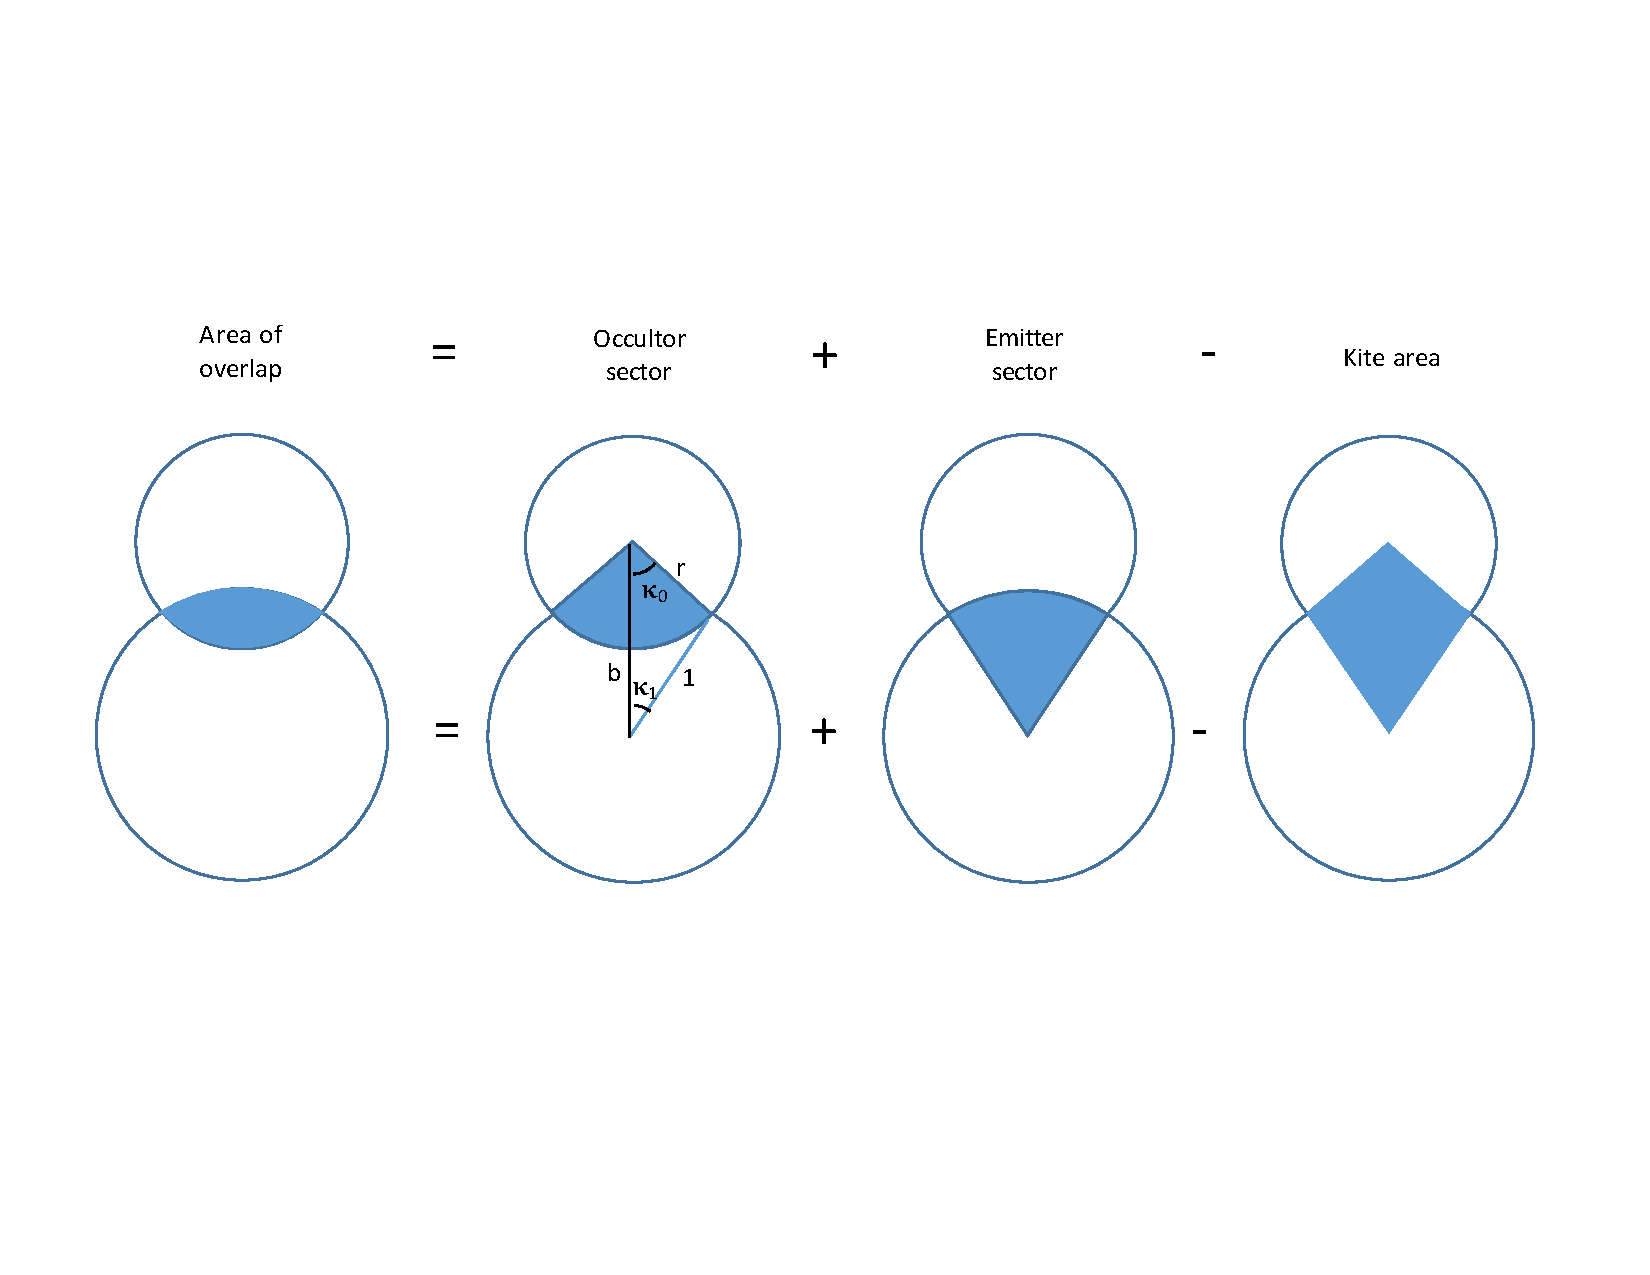
\includegraphics[width=\linewidth]{Circle_overlap_area.pdf}
    \caption{The area of overlap of two circles can be computed as the sum of
    the area of the sectors formed by the centers of each circle and the
    boundary between the points of intersection, minus the area of the kite-shaped
    region formed by the centers of the circles and the intersection points.}\label{fig:circle_overlap}
    \end{centering} 
\end{figure}

\begin{figure}
    \begin{centering}
    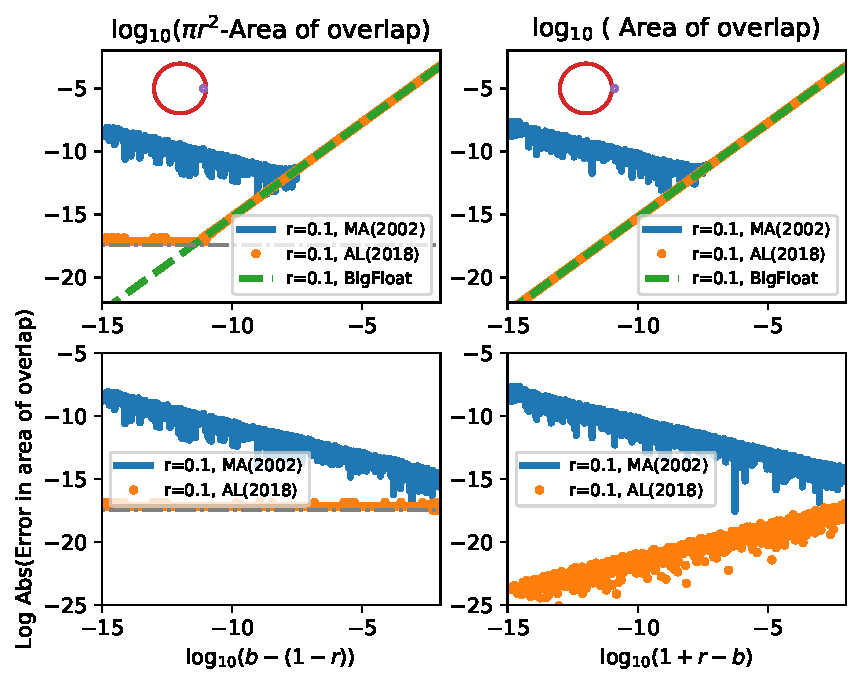
\includegraphics[width=\linewidth]{figures/julia/area_of_overlap.pdf}
    \caption{Precision of formulae for the area of overlap of two circles with
    radius ratio $r$.  Plotted are the regions near $b=1-r$ (second and third
    points of contact) and $b=1+r$ (first and fourth points of contact) for
    the standard formula (equation \ref{eq:MAuniform}, blue) and our new formula 
    (equation \ref{eq:area_of_overlap}, green). 
    The high-precision calculation is shown in red for comparison. The
    cyan and magenta circles indicate the positions of the circles at the left
    hand side of the axes.  In the left panels the dash-dot grey line indicates the 
    limiting precision for representing $\pi r^2$.}\label{fig:overlap_precision}
    \end{centering}
\end{figure}

\section{Linear Limb-Darkening}
\label{sec:reparam}
% ------------------------------------------------------------------------------
% ------------------------------------------------------------------------------
% ==============================================================================

In this section we turn to the case of linear limb-darkening, $I(\upmu) = \upmu$.
Note that since $\upmu = \sqrt{1-x^2-y^2}$, this problem is equivalent to 
computing the volume of intersection between a sphere and a cylinder, which was
solved in terms of elliptic integrals by \citet{Lamarche1990}.
A similar solution was found by \citet{MandelAgol2002}, who show that the total 
flux visible during the occultation of a body whose surface map is given by 
$I(x, y) = \sqrt{1 - \x^2 -\y^2}$ may be computed as
%
\begin{align}
    \label{eq:s2}
    S_1 = \frac{2\pi}{3} \left(1 - \frac{3\Lambda(r,b)}{2} - \Theta(r - b) \right)
\end{align}
%
where $\Theta(\bigdot)$ is the Heaviside step function and
%
\begingroup\makeatletter\def\f@size{10}\check@mathfonts
\def\maketag@@@#1{\hbox{\m@th\large\normalfont#1}}%
\begin{align}
    \label{eq:biglam}
    \Lambda(r,b) &=
    \begin{dcases}
          % I don't think we need this: the k^2>1 term is stable as b --> 0!
          %-\frac{2}{3}\left(1 - r^2\right)^\frac{3}{2}
          %& \qquad b = 0
          %
          %\\[1.5em]
          %
          \frac{1}{9 \pi \sqrt{b r}} \Bigg[
                \frac{(r + b)^2 - 1}{r + b}
                \Big(
                    -2r \,
                    \big(
                        2 (r + b)^2 + (r + b)(r - b) - 3
                    \big)
                    K(k^2)
                    &\\ \phantom{XXXX}
                    + 3 (b - r) \, \Pi\big(k^2 (b + r)^2, \, k^2\big)
                \Big)
                - 4 b r (4 - 7 r^2 - b^2) E(k^2)
          \Bigg]
          %
          & \qquad k^2 < 1
          %
          \\[1.5em]
          %
          \frac{2}{9 \pi} \Bigg[
                \big(1 - (r + b)^2\big)
                \Bigg(
                    \sqrt{1 - (b - r)^2} \,
                    K\left(\frac{1}{k^2}\right)
                    + 3 \left(\frac{b-r}{(b+r)\sqrt{1 - (b - r)^2}}\right)
                    &\\ \phantom{XX}
                    \times \Pi\left(\frac{1}{k^2(b+r)^2}, \, \frac{1}{k^2}\right)
                \Bigg)
                - \sqrt{1 - (b - r)^2}
                (4 - 7 r^2 - b^2)
                E\left(\frac{1}{k^2}\right)
          \Bigg]
          %
          & \qquad k^2 \ge 1
    \end{dcases}
\end{align}
\endgroup
%
with
%
\begin{align}
    \label{eq:k2}
    k^2 &= \frac{1 - r^2 - b^2 + 2 b r}{4 b r}
    \quad.
\end{align}
Note that $S_1 = s_2$ in the spherical harmonic expansion used in \starry as
described in Luger et al. (2018).
For the cases $b=r$, $b=1-r$, $b=0$, $r=0$, or $\vert r-b\vert \ge 1$, there are special
expressions for $\Lambda(r,b)$ given below.
%
In the expressions above, $K(\bigdot)$, $E(\bigdot)$, and $\Pi(\bigdot, \bigdot)$
are the complete elliptic integrals of the first, second kind, and third kind,
respectively, defined as
%
\begin{align}
    \label{eq:elliptic}
    K(k^2) &\equiv \int_0^{\frac{\pi}{2}} \frac{\dd \varphi}{\sqrt{1 - k^2 \sin^2 \varphi}}
    \nonumber \\[0.5em]
    E(k^2) &\equiv \int_0^{\frac{\pi}{2}} \sqrt{1 - k^2 \sin^2 \varphi} \, \dd \varphi
    \nonumber \\[0.5em]
    \Pi(n, k^2) &\equiv \int_0^{\frac{\pi}{2}} \frac{\dd \varphi}{(1 - n \sin^2 \varphi)\sqrt{1 - k^2 \sin^2 \varphi}}
    \quad.
\end{align}
In these expressions we have transformed the formulae from \citet{MandelAgol2002} using 
equation 17.7.17 from \citet{Abramowitz1970} which yields equations that are better
behaved in the vicinity of $b=r$.\footnote{Note that we corrected several typos
in \citet{MandelAgol2002}, which are listed in the Appendix.}  However, these elliptic 
integrals are still subject to numerical instability as $r \rightarrow 1-b$ and $r \gg 1$.  
The main issue is the logarithmic divergence of $K$ and $\Pi$ as $k \rightarrow 1$, as
well as numerical cancellations leading to round-off errors which occur in the 
limit $k \rightarrow 0$.

Through trial and error, we have found that these instabilities can be removed by combining
elliptic integrals into a general complete elliptic integral defined by \citet{Bulirsch1969} as
\begin{equation}
{\rm cel}(k_c,p,a,b) = \int_0^{\pi/2} \frac{a\cos^2{\phi} + b\sin^2{\phi}}{\cos^2{\phi}+p\sin^2{\phi}} \frac{d\phi}{\sqrt{\cos^2{\phi}+k_c^2\sin^2{\phi}}},
\end{equation}
where $k_c = \sqrt{1-m}$ where for $b+r \ge 1$,
$m=k^2$, while for $b+r \le 1$, $m=1/k^2$.  Although $k_c$ can be computed from
$m$, we have found better numerical stability in computing $k_c$ analytically
from $b$ and $r$, rather than from $m$:
\begin{align}
    k_c &=
    \begin{dcases}
     \sqrt{\frac{(b+r)^2-1}{4br}} & \qquad k^2 \le 1\\
     \sqrt{\frac{1-(b+r)^2}{1-(b-r)^2}} & \qquad k^2 > 1.
   \end{dcases}
\end{align}
In practice, we let the subroutine that computes ${\rm cel}$ accept both
$m$ and $k_c$ as input for numerical precision.

To transform the elliptic integrals in equation \ref{eq:biglam},
we used the following relations from \citet{Bulirsch1969}:
\begin{eqnarray}
\lambda K(m) + q E(m) &=& {\rm cel}(k_c,1,\lambda+q,\lambda+q k_c^2)\\
\lambda K(m) + q \Pi(n,m) &=& {\rm cel}(k_c,1-n,\lambda+q,\lambda+q k_c^2)\\
E(m) &=& {\rm cel}(k_c,1,1,1-m)\\
E(m)-(1-m)K(m) &=& m \, {\rm cel}(k_c,1,1,0)\\
\Pi(n,m)-K(m)  &=& n \, {\rm cel}(k_c,1-n,0,1),
\end{eqnarray}
noting that \citet{Bulirsch1969} uses a different sign convention for $\Pi(n,m)$.
In particular, the expressions for $\Pi(n,m)-K(m)$ and $E(m)-(1-m)K(m)$ are useful for eliminating
the singularities and cancellations which occur at $m=1$ when $b+r=1$ and $m=0$ when
$r \rightarrow \infty$.  The general complete elliptic integral is evaluated
with the approach of \citet{Bartky1938}, which uses recursion to approximate the
integral to a specified precision.

These elliptic integral transformations lead to the following numerically-stable
expression for the linear limb-darkening flux, $s_2(r,b) = S_1(r,b)$, in which
\begin{align}
    \label{eq:biglam_stable}
    \Lambda &=
    \begin{dcases}
          0 & \qquad  r = 0\\
          0 & \qquad  \vert r- b\vert \ge 1\\
          -\tfrac{2}{3}(1-r^2)^{3/2} & \qquad b = 0\\
          \tfrac{1}{3} - \tfrac{4}{9\pi} & \qquad b = r = \tfrac{1}{2}\\
          \tfrac{1}{3} + \tfrac{2}{9\pi} {\rm cel}\left(k_c,1,m-3,(1-m)(2m-3)\right) & \qquad b= r < \tfrac{1}{2}\\
          \tfrac{1}{3} + \tfrac{1}{9\pi r} {\rm cel}\left(k_c,1,m-3,1-m\right) & \qquad b= r > \tfrac{1}{2}\\  % I think this equation may have a mistake [ ]  EA 7/17/2018
          \tfrac{2}{9\pi}\left[3\cos^{-1}(1-2r) -2(3+2r-8r^2)\sqrt{rb}-3\pi\Theta(r-\tfrac{1}{2})\right] & \qquad b+r =1\\
          \frac{1-(b-r)^2}{9 \pi \sqrt{b r}} \Bigg[
                \frac{(b+r)^2-1}{4br}(b^2-r^2){\rm cel}(k_c,(b-r)^2(1-m),0,3)
                &\\ \phantom{XXXX}
               - (3-6r^2-2br){\rm cel}(k_c,1,1,0)-4brE(m)
          \Bigg]
          %
          & \qquad k^2 < 1
          %
          \\[1.5em]
          %
          \frac{2\sqrt{1-(b-r)^2}}{9 \pi} \Bigg[
                \big(1 - (r + b)^2\big)
                {\rm cel}(k_c,p,1+q,p+q) &\\ \phantom{XXXX}
                - (4 - 7 r^2 - b^2)
                E\left(m\right)
          \Bigg]
          %
          & \qquad k^2 > 1\\
    \end{dcases}
\end{align}
where
\begin{eqnarray}
q &=& 3\frac{b-r}{(b+r)(1-(b-r)^2)}\\
p &=& \left(\frac{b-r}{b+r}\right)^2 \frac{1-(b+r)^2}{1-(b-r)^2}
\end{eqnarray}
in the $k^2 > 1$ case.  Note that in this equation the conditions
should be evaluated in the order they appear.

The $s_2(r,b)$ function is plotted in Figure \ref{s2_plot}.  The
function varies smoothly from the lower right where the disk is
unocculted to the upper left where it is completely occulted.
There are several points which need to be handled separately as
the equation \ref{eq:biglam} expressions become singular or are
no longer valid;  the solid lines in Figure \ref{s2_plot} show
these points.  When $b=0$, the integral over the center of the
disk simplifies greatly.  When $b=r=1/2$, at the intersection of
$b=r$ and $b=1-r$, another simplification occurs.  For $b=r$,
the disk of the occultor crosses the center of the source;
this needs to be computed separately in the $r<1/2$, $r=1/2$,
and $r>1/2$ limits.  The first and fourth contacts occur at
$b=1+r$, where $s_2=1$;  this is the upper bound to the $k^2 < 1$
region for $b+r >1$.
For $r \ge 1$, the second and third contacts (at the start and
end of complete occultation) occur when $b=1-r$, which is the
lower  bound to the $k^2<1$ region when $b+r >1$.
For $r < 1$, the second and third contacts occur when $r=1-b$.

Near these boundaries, the standard \citet{MandelAgol2002} expressions
can become singular, and so we paid particular care to the accuracy of these
new expressions in these regions.  Figure \ref{s2_machine} shows
that equation \ref{eq:biglam_stable} is accurate to machine
precision in all of these regimes.
We tested the accuracy by computing the equations with 256 bit
arithmetic, which is much less subject to round-off error, and
hence gives essentially exact expressions.  We implemented the
pseudocode from \citet{Bulirsch1969} to compute ${\rm cel}(k_c,p,a,b)$,
which has a termination test that scales as the square root of
the machine precision.  We find that the transformed expressions
are accurate to $\la \times 10^{-14}$ when computed in double precision
within $10^{-8}$ of the vicinity of $b=r$ and $b=1-r$.

\begin{figure}\label{transit_linear}
    \begin{centering}
    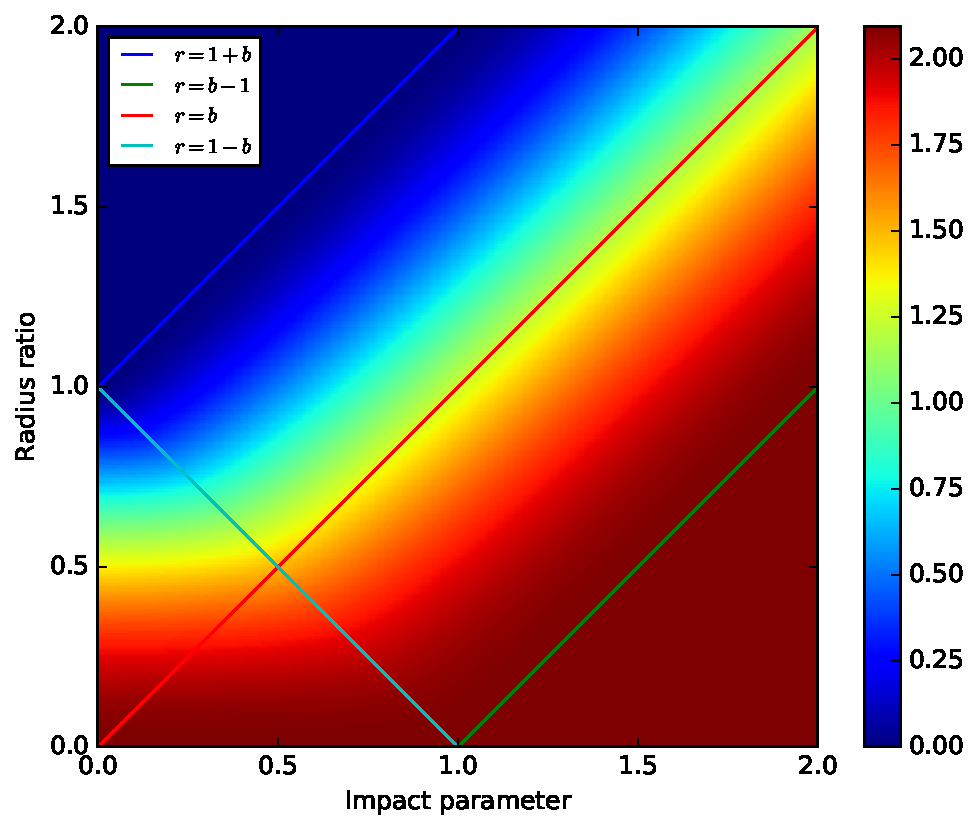
\includegraphics[width=0.85\linewidth]{figures/julia/transit_linear.pdf}
    \caption{The intensity of a linearly limb-darkened star ($u_1=1$) being
    eclipsed, $s_2(r,b)$.
    In the limit $b > r+1$, no eclipse occurs, so $s_2=1$.  For $b < r-1$, the star
    is completely eclipsed and $s_2=0$.  In the limits $b=r$ and $b=1-r$, special
    expressions must be used}
    \end{centering}
\end{figure}

\begin{figure}\label{s2_plot}
    \begin{centering}
    \includegraphics[width=0.85\linewidth]{figures/julia/s2_residuals.pdf}
    \caption{The numerical error in computing the flux of an eclipsed,  linearly
    limb-darkened star ($u_1=1$), $s_2(r,b)$.}
    \end{centering}
\end{figure}

\begin{figure}\label{s2_machine}
    \begin{centering}
    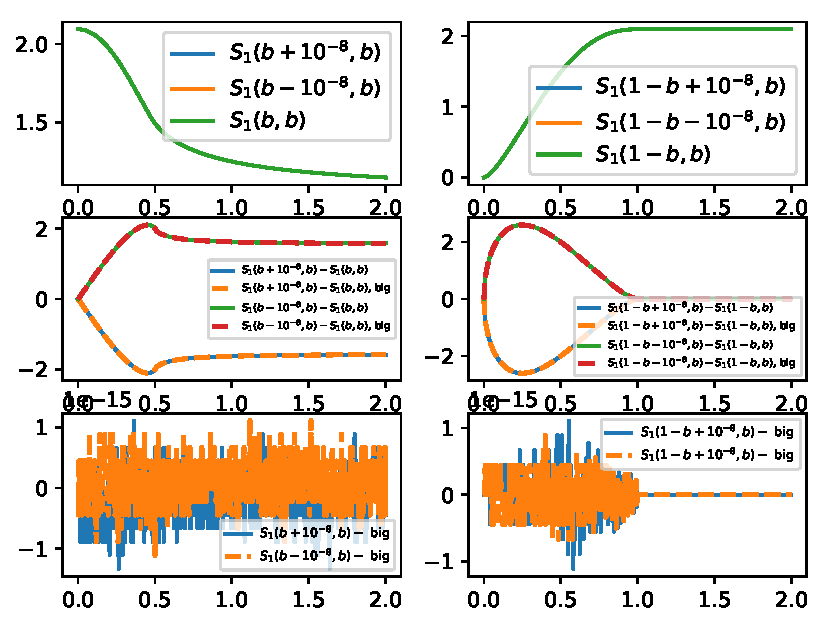
\includegraphics[width=\linewidth]{figures/julia/s2_machine.pdf}
    \caption{The accuracy of $s_2(r,b)$ near $b=r$ (left panel) and
    $b=1-r$ (right panel). The x-axese are impact parameter b,
    while the y axes in the top panels show $s_2(r,b)$, with $r$
    given in the legend of each panel. The middle panels plot
    the difference $(s_2(b,b\pm\epsilon)-s_2(b,b))/\epsilon$
    and $(s_2(b,1-b\pm\epsilon)-s_2(b,1-b))/\epsilon$. The bottom
    panels show the numerical precision by the comparing double precision
    computation with \texttt{BigFloat} precision (256-bit).}
    \end{centering}
\end{figure}


From \citet{MandelAgol2002}, the total flux visible during the occultation of a
body whose surface map is given by $I(\upmu)/I(1) = 1 - u_1(1 - \upmu)$ may be computed
as
\begin{eqnarray}
\frac{F(u_1,r,b)}{F_0} &=& \frac{\pi(1-u_1)(1-\Lambda^e)+ u_1 S_1(r,b)}{\frac{2\pi}{3}u_1 + \pi(1-u_1)},\\
&=& 1-(1-u_1/3)^{-1}\left[(1-u_1)\Lambda^e(r,b) + u_1\left(\Lambda(r,b)+\tfrac{2}{3}\Theta(r-b)\right)\right],
\end{eqnarray}
where
and $F_0$ is the total unocculted flux.  % Note:  I'm not using this in 
% transit_poly since it is not as precise as the starry expressions.

\subsection{Derivatives of linear limb-darkening}

It turns out that the expressions for the derivatives of the linear limb-darkening
light curve with respect to $r,b$ are particularly simple:
\begin{align}
    \label{eq:dbiglam_dr}
    \frac{\partial \Lambda}{\partial r} &=
    \begin{dcases}
          0 & \qquad  r = 0\\
          0 & \qquad  \vert r- b\vert \ge 1\\
          2 r\sqrt{1-r^2} & \qquad b = 0\\
           \frac{2}{\pi} & \qquad b = r = \tfrac{1}{2}\\
          \frac{4r}{\pi} E(4r^2) & \qquad b= r < \tfrac{1}{2}\\
          \frac{2}{\pi} \mathrm{cel}(k_c,1,1,0) & \qquad b= r > \tfrac{1}{2}\\
          \frac{8r}{\pi}\sqrt{r(1-r)} & \qquad b+r =1\\
          \frac{8br^2 E(k^2) + 2r(1-(b+r)^2)K(k^2)}{\pi\sqrt{br}}
                    &\\ \phantom{XX}
          = \frac{1}{\pi\sqrt{br}}\mathrm{cel}(k_c,1,2r(1-(b-r)^2),0) & \qquad k^2 < 1
          %
          \\[1.5em]
          %
          \frac{4r}{\pi}\sqrt{1-(b-r)^2} E(k^{-2})
                    &\\ \phantom{XX}
          = \frac{4r}{\pi}\sqrt{1-(b-r)^2} \mathrm{cel}(k_c,1,1,k_c^2)& \qquad k^2 > 1\\
    \end{dcases}
\end{align}
and
\begin{align}
    \label{eq:dbiglam_db}
    \frac{\partial \Lambda}{\partial b} &=
    \begin{dcases}
          0 & \qquad  r = 0\\
          0 & \qquad  \vert r- b\vert \ge 1\\
          0 & \qquad b = 0\\
           -\frac{2}{3\pi} & \qquad b = r = \tfrac{1}{2}\\
          \frac{4r}{3\pi}\mathrm{cel}(k_c,1,-1,k_c^2) & \qquad b= r < \tfrac{1}{2}\\
          -\frac{2}{3\pi} \mathrm{cel}(k_c,1,1,2k_c^2) & \qquad b= r > \tfrac{1}{2}\\
          -\frac{8r}{3\pi}\sqrt{r(1-r)} & \qquad b+r =1\\
           \frac{4r(r^2+b^2-1) E(k^2) + 2r(1-(b+r)^2)K(k^2)}{3\pi\sqrt{br}} 
                    &\\ \phantom{XX}
          = \frac{1-(b-r)^2}{3\pi \sqrt{br}} \mathrm{cel}(k_c,1,-2r,(1-(b+r)^2)/b) & \qquad k^2 < 1
          %
          \\[1.5em]
          %
          \frac{2}{3b\pi}\sqrt{1-(b-r)^2}\left[(r^2+b^2-1) E(k^{-2}) +(1-(b+r)^2)K(k^{-2})\right]
                    &\\ \phantom{XX}
          =\frac{4r}{3\pi}\sqrt{1-(b-r)^2}\mathrm{cel}(k_c,1,-1,k_c^2) & \qquad k^2 > 1,\\
    \end{dcases}
\end{align}
where we have given some of the expressions in terms of both the standard elliptic integrals
and the general elliptic integral.

Note that if we had included the radius of the source star in these formulae,
then the derivatives with respect to the radius of the star yield the
transit light curve of a uniform emission shell \citep{Schlawin2010}.

We have tested these formulae with finite-difference derivatives evaluated at
256-bit precision, and, as with the total flux term, we find that these are accurate 
to $\la 2 \times 10^{-15}$, close to machine precision.

Finally, we turn our attention to the general polynomial limb-darkening case,
$\upmu^n$ with $n \ge 2$.  These terms may be expressed as the sum of
spherical harmonics with $m=0$, and thus they are a special case of the \starry 
computation (written in C and Python), which we describe next in \S \ref{sec:quad}.  
We have also derived a new approach exploiting the azimuthal symmetry of the 
limb-darkening problem, which we describe below in \S \ref{sec:power_law}, 
which is implemented in \texttt{Julia}.

%\begin{eqnarray}
%\frac{\partial \Lambda}{\partial r} &=& \frac{8br^2 E(k^2) + 2r(1-(b+r)^2)K(k^2)}{\pi\sqrt{br}}\\ 
%&=& \frac{1}{\pi\sqrt{br}}\mathrm{cel}(k_c,1,2r(1-(b-r)^2),0)\\ 
%\frac{\partial \Lambda}{\partial b} &=& \frac{4r(r^2+b^2-1) E(k^2) + 2r(1-(b+r)^2)K(k^2)}{3\pi\sqrt{br}}\\ 
%&=& \frac{1-(b-r)^2}{3\pi \sqrt{br}} \mathrm{cel}(k_c,1,-2r,(1-(b+r)^2)/b)\\ 
%\frac{\partial \Lambda}{\partial r} &=& \frac{4r}{\pi}\sqrt{1-(b-r)^2} E(k^{-2})\\ 
%&=& \frac{4r}{\pi}\sqrt{1-(b-r)^2} \mathrm{cel}(k_c,1,1,k_c^2)\\ 
%\frac{\partial \Lambda}{\partial b} &=& \frac{2}{3b\pi}\sqrt{1-(b-r)^2}\left[(r^2+b^2-1) E(k^{-2}) +(1-(b+r)^2)K(k^{-2})\right]\\ 
%&=& \frac{4r}{3\pi}\sqrt{1-(b-r)^2}\mathrm{cel}(k_c,1,-1,k_c^2)
%\end{eqnarray}

% ==============================================================================
% ------------------------------------------------------------------------------
% ------------------------------------------------------------------------------
%
\clearpage
\section{Polynomial Limb-Darkening}
\label{sec:quad}
% ------------------------------------------------------------------------------
% ------------------------------------------------------------------------------
% ==============================================================================

In analogy with the linear and quadratic
limb-darkening laws, let us define the polynomial limb-darkening law of
order $l_\mathrm{max}$ as
%
%
\begin{align}
    \label{eq:polynomialld}
    \frac{I(\upmu)}{I(1)} &= 1 - u_1 (1 - \upmu) - u_2 (1 - \upmu)^2 - ... - u_{l_\mathrm{lmax}}(1 - \upmu)^{l_\mathrm{lmax}} \nonumber \\
                          &= \sum_{l=0}^{l_\mathrm{lmax}} \sum_{k=0}^l u_l {l \choose k} (-1)^k \upmu^k
    \quad,
\end{align}
%
where $u_0 \equiv 1$. For convenience, this can be expressed as the matrix equation
%
\begin{align}
    \label{eq:polynomialldmatrix}
    \frac{I(\upmu)}{I(1)} &= \bvec{u}^\top \, \bvec{L} \, \pmb{\upmu}
    \quad,
\end{align}
%
where $\bvec{u}^\top$ is a row vector whose value at index
$l$ is $u_l$, $\pmb{\upmu}$ is a column vector whose value at index $k$ is $\upmu^k$,
and $\bvec{L}$ is the lower triangular matrix with components given by
%
\begin{align}
    \label{eq:Llk}
    L_{lk} = {l \choose k} (-1)^k
    \quad.
\end{align}
%
It is straightforward to show that this law can be
expressed exactly as a sum over the $m = 0$ spherical harmonics, which also
form a complete basis of radially symmetric functions on the sphere.
%
Based on the relations in \citet{starry} for the spherical harmonics in Cartesian
form, the spherical harmonics of order $m = 0$ may be written
%
\begin{align}
    \label{eq:Ylzero}
    Y_{l,0}(\upmu) = \sqrt{\frac{2l + 1}{4\pi}}
              \sum_{k=0}^l {l \choose k} \frac{(k + l - 1)!!}{(k - l - 1)!!} \upmu^k
\end{align}
%
where $\upmu = z = \sqrt{1 - x^2 - y^2}$, $\binom{\bigdot}{\bigdot}$ is a binomial
coefficient, and $!!$ denotes the double factorial.

Our task now is to express the specific intensity function (\ref{eq:polynomialldmatrix})
in the basis of spherical harmonics (\ref{eq:Ylzero}). We therefore wish to find
the coefficients $c_l$ for which we may write
%
\begin{align}
    \label{eq:sphharmld}
    \frac{I(\upmu)}{I(1)} &= \sum_{l=0}^{l_\mathrm{lmax}} c_l Y_{l,0}(\upmu)
    \quad.
\end{align}
%
As before, we can write this as the matrix equation
%
\begin{align}
    \label{eq:sphharmldmatrix}
    \frac{I(\upmu)}{I(1)} &= \bvec{c}^\top \, \bvec{M} \, \pmb{\upmu}
    \quad,
\end{align}
%
where $\bvec{c}^\top$ is a row vector whose value at index
$l$ is $c_l$ and $\bvec{M}$ is the lower triangular matrix with components given by
%
\begin{align}
    \label{eq:Mlk}
    M_{lk} = \sqrt{\frac{2l + 1}{4\pi}} {l \choose k} \frac{(k + l - 1)!!}{(k - l - 1)!!}
    \quad.
\end{align}
%
Equating Equations~(\ref{eq:polynomialldmatrix}) and (\ref{eq:sphharmldmatrix}), we see
that we must have
%
\begin{align}
    \bvec{c}^\top \, \bvec{M} = \bvec{u}^\top \, \bvec{L} \quad,
\end{align}
%
or
%
\begin{align}
    \bvec{c} = (\bvec{M}^{-1} \, \bvec{L})^\top \bvec{u} \quad.
\end{align}
%
In \citet{starry} we described how to compute analytic transit and occultation light curves
for bodies whose surfaces are expressed as a sum over spherical harmonic coefficients. We
defined a body's surface map as the vector of spherical harmonic coefficients $\bvec{y}$.
The vector $\bvec{y}$ corresponding to our coefficients for the $Y_{l,0}$ harmonics is
related to $\bvec{c}$ via
%
\begin{align}
    y_{l(l + 1)} &= c_l
\end{align}
%
for $0 \leq l \leq l_\mathrm{max}$, where the values at all other indices in $\bvec{y}$ are zero.

\begin{figure}[t!]
    \begin{centering}
    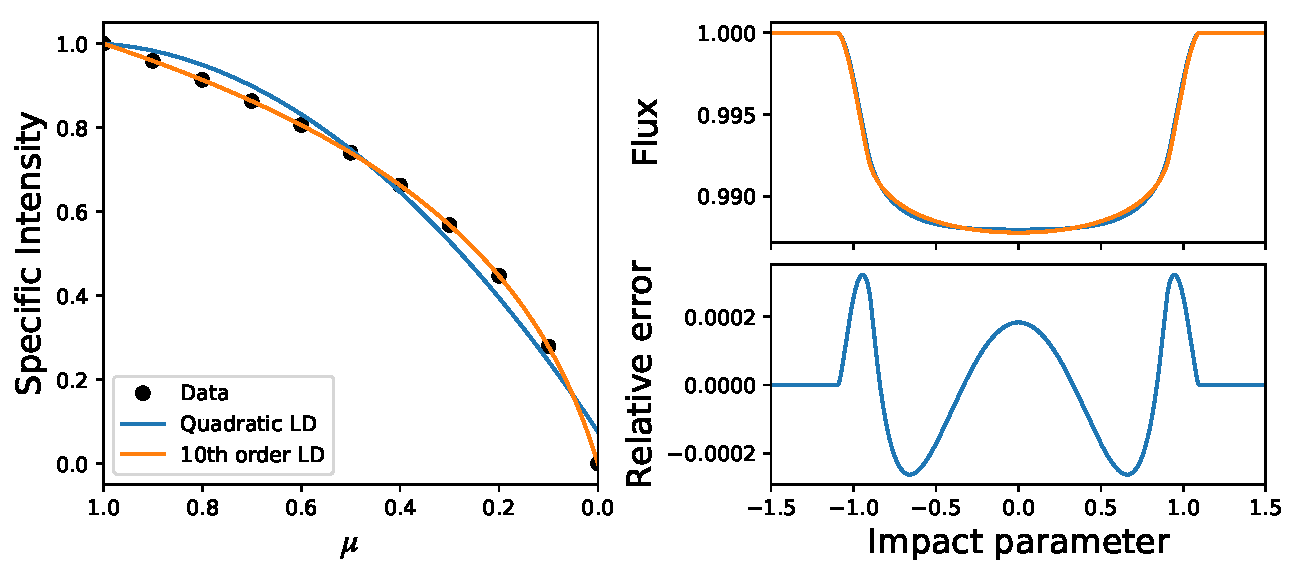
\includegraphics[width=\linewidth]{figures/python/high_order_ld.pdf}
    \caption{\label{fig:high_order_ld} Tenth order limb-darkening example with \starry. }
    \end{centering}
\end{figure}

{\color{red}We should derive simplified expressions of our formulae in \starry for the $m = 0$ case.} \todo{}

\begin{align}
    \label{eq:PGnI}
    \mathcal{P}(\bvec{G}_n) &=
    \begin{dcases}
        %
        r^{l+2} \sum\displaylimits_{i=0}^{\frac{l}{2}}
                {\frac{l}{2} \choose i}
                \left(\frac{b}{r}\right)^{\frac{l-2i}{2}}
                \mathcal{I}_{\frac{l+4}{2}, i}
            %
            & \qquad \frac{l}{2} \, \mathrm{even}
        \\[1em]
        %
        -r^{l-2} \left( b \mathcal{J}_{l-3,1} + r \mathcal{J}_{l-3,2} \right)
        %
        & \qquad l = 1
        \\[1em]
        %
        r^{l-1} \sum\displaylimits_{i=0}^{\frac{l-1}{2}}
                {\frac{l-1}{2} \choose i}
                \left(\frac{b}{r}\right)^{\frac{l-2i-1}{2}}
                \mathcal{J}_{\frac{l-1}{2}, i}
            & \qquad \frac{l-1}{2} \, \mathrm{even}
        \\[1em]
        %
        0 & \qquad \mathrm{otherwise}
    \end{dcases}
%
\end{align}
%
\begin{align}
%
    \nonumber \\
    \label{eq:QGnI}
    \mathcal{Q}(\bvec{G}_n) &=
    \begin{dcases}
        \mathcal{H}_{\frac{l+4}{2}, \frac{l}{2}}
        & \qquad \qquad \qquad \qquad \quad \quad \quad \quad \frac{l}{2} \, \mathrm{even}
        \\[1em]
        %
        0
        & \qquad \qquad \qquad \qquad \quad \quad \quad \quad \mathrm{otherwise} \quad.
    \end{dcases}
\end{align}

We have computed derivatives of these expressions using automatic
differentiation within the \starry code base.

\section{Alternative Green's function expansion} \label{sec:power_law}

Although the foregoing analysis takes advantage of the existing formalism
developed for occultation of spheres with arbitrary spherical harmonic
brightness, the problem can be simplified somewhat for the limb-darkening
case due to azimuthal symmetry assumed for a star.  This simplification
leads to analytic expressions for the derivatives, which we find can be 
faster and more accurate to evaluate than with automatic differentiation.

Since the polynomial expansion only depends on $\upmu = z =\sqrt{1-x^2-y^2}$,
where $(x,y,z)$ are the coordinates of the unit sphere, then we only require
Green's functions whose curl has dependence only on $z$ for axially-symmetric
limb-darkening.  Following Luger et al. (2018), we choose a Green's function 
of the form
\begin{equation}
\mathbf{G}_n = f(z) (-y \xhat + x \yhat)
\end{equation}
giving
\begin{eqnarray}
\gbasisn(x,y) &=& \frac{\dd {G_n}_y}{\dd \x} - \frac{\dd {G_n}_x}{\dd \y}\\
&=& 2 f(z) + \frac{df}{dz} \frac{z^2-1}{z}.
\end{eqnarray}
This yields particularly simple form for the primitive integrals of
\begin{align}
    \label{eq:primitiveP}
    \mathcal{P}(\bvec{G}_n) &=
    \int\displaylimits_{\pi-\phi}^{2\pi + \phi} f(z) (r+b \sin{\varphi}) r d\varphi
    %
\intertext{and}
    %
    \label{eq:primitiveQ}
    \mathcal{Q}(\bvec{G}_n) &=
    \int\displaylimits_{\pi-\lambda}^{2\pi + \lambda} f(z) d \varphi
\end{align}

We choose $f(z) = z^n$, so that
\begin{equation}
\gbasisn(x,y) =  (n+2)z^n-n z^{n-2},
\end{equation}
is the basis set for the surface brightness of the polynomial limb-darkening, 
along with the uniform, $\tilde{g}_0 = z^0$,
and linear, $\tilde{g}_1 = z^1$, terms which we have derived in \S \ref{sec:reparam}.
Note that the total flux of each term in this basis set, $\tilde{g}_n$, integrates
to a total flux of zero for $n \ge 2$.

Also, with this choice of basis, the primitive integral $\mathcal{Q}(\bvec{G}_n) = 0$ for 
$n \ge 1$ since $z=0$ at the boundary of the star.   The $n=0$ case we have already
solved for uniform limb-darkening, and so it remains to find $\mathcal{P}(\bvec{G}_n)$.

The primitive integral
$\mathcal{P}(\bvec{G}_n)$ can be rewritten as
\begin{equation}
\mathcal{P}(\bvec{G}_n) = 
\int_{\pi-\phi}^{2\pi + \phi} \left(1-r^2-b^2-2br s_\varphi\right)^{\frac{n}{2}} (r+b s_\varphi) r d\varphi,
\end{equation}
where $s_\varphi = \sin{\varphi}$.
We make the transformation $\xi = \tfrac{1}{2} \left(\varphi - \tfrac{3\pi}{2}\right)$, yielding
\begin{equation}
\mathcal{P}(\bvec{G}_n) = 
2r (4br)^{\frac{n}{2}}\int\displaylimits_{-\tfrac{\kappa}{2}}^{\tfrac{\kappa}{2}} 
(k^2-\sin^2\xi)^{\tfrac{n}{2}} (r-b + 2b \sin^2 \xi) d\xi,
\end{equation}
for even values of $n$ and 
\begin{equation}
\mathcal{P}(\bvec{G}_n) =
2r (4br)^{\frac{n}{2}} k^3 \int\displaylimits_{-\tfrac{\kappa}{2}}^{\tfrac{\kappa}{2}} 
(k^2-\sin^2\xi)^{\tfrac{n-3}{2}} (1-k^{-2} \sin^2 \xi)^{3/2} (r-b + 2b \sin^2 \xi) d\xi,
\end{equation}
for odd values of $n \ge 3$, where $\kappa = 2 \cos^{-1}k$ for $k^2 \le 1$ and
$\kappa = \pi$ for $k^2 > 1$.

Each of the terms $(k^2-\sin^2\xi)^c$ can be expanded with the binomial theorem,
and then expressed in terms of the integrals $\mathcal{I}_v(k)$ and $\mathcal{J}_v(k)$ 
(defined in Luger et al. 2018) as
\begin{eqnarray}
\mathcal{P}(\mathbf{G}_n)
= 2r(4br)^{n_0} \sum_{i=0}^{n_0} \binom{n_0}{i}(-1)^{n_0-i} k^{2i} \left[(r-b)\mathcal{I}_{n_0-i} + 2b \mathcal{I}_{n_0-i+1}\right],
\end{eqnarray}
for even $n$, where $n_0 = n/2$, and
\begin{eqnarray}
\mathcal{P}(\mathbf{G}_n) 
= \mathcal{F}(4br)^{n_0} \sum_{i=0}^{n_0} \binom{n_0}{i} (-1)^{n_0-i} k^{2i} \left[(r-b)\mathcal{J}_{n_0-i} + 2b \mathcal{J}_{n_0-i+1}\right],
\end{eqnarray}
for odd $n \ge 3$, where $n_0 = (n-3)/2$ and
 $\mathcal{F} = 2r(1-(b-r)^2)^{3/2}$.

\subsection{Limb-darkening coefficients}

Our expansion for limb-darkening in terms of $u_n(1-\upmu)^n$ needs to
be re-expressed in terms of the Green's basis terms $d_n \left[(n+2)\upmu^n -n \upmu^{n-2}\right]$.
We accomplish this by first transforming $u_n$ to coefficients of $a_n \upmu^n$,
and then transforming from $a_n$ to $d_n$.

We rewrite $I(\upmu)$ in terms of these three expansions
\begin{eqnarray}
I(\upmu) &=& 1 - \sum_{i=1}^N u_i \sum_{j=0}^i \binom{i}{j} (-1)^j \upmu^j,\\
&=& \sum_{n=0}^N a_n \upmu^n,\\
&=& d_0 + d_1 \upmu + \sum_{n=2}^N d_n \left[(n+2)\upmu^n -n \upmu^{n-2}\right].
\end{eqnarray}
Note that $a_0= 1-\sum_{n=1}^N a_n = 1 - \sum_{i=1}^N u_i$ in the formalism of \citet{Gimenez2006}.
The transformation between $u_n$ and $a_n$ is straightforward based on
looping over the binomial expansion of each of the $u_n$ terms (equation \ref{eq:polynomialld}),
for example $a_1 = \sum_{n=1}^N n u_n$.
Then, with the computed $a_n$ values, we can find $d_n$ from downward recursion
using the relation
\begin{equation}
d_n = \frac{a_n}{n+2} + d_{n+2},
\end{equation}
starting with $n=N$, with $d_{N+1}=d_{N+2}=0$.

The total light curve is computed from
\begin{eqnarray}
\frac{F}{F_0} &=& \frac{1}{F_0}\sum_{n=0}^N d_n S_n,\\
F_0 &=& \pi(d_0+ \tfrac{2}{3} d_1),
\end{eqnarray}
where $F_0$ is the unobscured flux, $S_0$ is given for uniform limb-darkening
in section \ref{eq:uniform}, $S_1=s_2$ is given by the linear limb-darkened 
solution from section \ref{sec:reparam}, and  $S_n = \mathcal{Q}(\bvec{G}_n) 
- \mathcal{P}(\bvec{G}_n)$ for $n \ge 2$.

We note that the unobscured flux for each basis function (for $b \ge 1+r$ or $r=0$) is zero for
all $S_n(r,b)$ with $n \ge 2$, which is why the total unobscured flux,
$F_0$, only depends upon $d_0$ and $d_1$.

\subsection{Analytic derivatives}

For computing the derivatives of $\mathcal{P}(\bvec{G}_n)$, we find it more numerically 
stable to express the $k^{2i}$ terms in terms of $b$ and $r$.  For compactness, we define
\begin{eqnarray}
T_i &=&  \binom{n_0}{i}(-4br)^{n_0-i}(1-(b-r)^2)^{2i},\\
U_i &=&  \left[(r-b)\mathcal{I}_{n_0-i} + 2b \mathcal{I}_{n_0-i+1}\right],\\
V_i &=&  \left[(r-b)\mathcal{J}_{n_0-i} + 2b \mathcal{J}_{n_0-i+1}\right],
\end{eqnarray}
so that we can rewrite the primitive integral as
\begin{eqnarray}
\mathcal{P}(\mathbf{G}_n) &=& 2r \sum_{i=0}^{n_0} T_i U_i\\
&=& \mathcal{F} \sum_{i=0}^{n_0} T_i V_i,
\end{eqnarray}
where the first line is for even $n$ and the second for odd $n \ge 3$.

We then express the derivatives as
\begin{eqnarray}
\frac{d \mathcal{P}}{d r} = \frac{\partial \mathcal{P}}{\partial r}  +  \frac{\partial \mathcal{P}}{\partial k} \frac{\partial k}{\partial r},\\
\frac{d \mathcal{P}}{d b} = \frac{\partial \mathcal{P}}{\partial b}  +  \frac{\partial \mathcal{P}}{\partial k} \frac{\partial k}{\partial b}.
\end{eqnarray}

Then, these partial derivatives are given by:
\begin{eqnarray}
\frac{\partial \mathcal{P}}{\partial r}  &=& 2r\sum_{i=0}^{n_0} T_i  \left[\left(\frac{2i(b-r)}{1-(b-r)^2} + \frac{n_0+1-i}{r}\right) U_i + \mathcal{I}_{n_0-i}\right],\\
\frac{\partial \mathcal{P}}{\partial b}  &=& 2r\sum_{i=0}^{n_0} T_i  \left[\left(\frac{2i(r-b)}{1-(b-r)^2} + \frac{n_0-i}{b}\right) U_i - \mathcal{I}_{n_0-i} + 2\mathcal{I}_{n_0-i+1}\right],\\
\frac{\partial \mathcal{P}}{\partial k}  &=& 0,
\end{eqnarray}
for even $n$ and
\begin{eqnarray}
\frac{\partial \mathcal{P}}{\partial r}  &=& \mathcal{F}\sum_{i=0}^{n_0} T_i \left[\left(\frac{(2i+3)(b-r)}{1-(b-r)^2} + \frac{n_0+1-i}{b}\right) V_i + \mathcal{J}_{n_0-i}\right],\\
\frac{\partial \mathcal{P}}{\partial b}  &=& \mathcal{F}\sum_{i=0}^{n_0} T_i \left[\left(\frac{(2i+3)(r-b)}{1-(b-r)^2} + \frac{n_0-i}{b}\right) V_i - \mathcal{J}_{n_0-i} + 2\mathcal{J}_{n_0-i+1}\right],\\
\frac{\partial \mathcal{P}}{\partial k}  &=& \mathcal{F}\sum_{i=0}^{n_0} T_i \left[(r-b) \frac{\partial\mathcal{J}_{n_0-i}}{\partial k} + 2b \frac{\partial \mathcal{J}_{n_0-i+1}}{\partial k}\right],
\end{eqnarray}
for odd $n \ge 3$.

The partial derivatives of $k$ are given by
\begin{eqnarray}
\frac{\partial k}{\partial r} &=& \frac{b^2-r^2-1}{8 k b r^2},\\
\frac{\partial k}{\partial b} &=& \frac{r^2-b^2-1}{8 k b^2 r}.
\end{eqnarray}

Finally, we need the derivatives of the function $\mathcal{I}_v$ and $\mathcal{J}_v$
with respect to $k$.  This is given by recursion relations
\begin{eqnarray}
\frac{\partial \mathcal{J}_v}{\partial k} &=& -3 k^{-1} \mathcal{J}_v +k^2 \frac{\partial \mathcal{J}_{v-1}}{\partial k},\\
&=& 3 k^{2v} \int_0^1 u^{v+\tfrac{1}{2}} (1-u)^{1/2} (1-k^2u)^{-1/2}du,\\ 
&=& 3 k^{2v} \frac{\sqrt{\pi}}{2} \Gamma(v+\tfrac{3}{2}) \,_2{\tilde F}_1(\tfrac{1}{2},v+\tfrac{3}{2},3+v,k^2),\\
\frac{\partial \mathcal{J}_0}{\partial k} &=& \frac{2}{k^4}\left[(2-k^2)E(k^2)+2(k^2-1)K(k^2)\right],
\end{eqnarray}
for $k^2 < 1$ ($b+r > 1$) and an expression for $I_v$
\begin{equation}
\frac{\partial \mathcal{I}_v}{\partial k} = 2k^{2v} k_c^{-1}.
\end{equation}

For $k^2 > 1$ ($b+r <1$), we have
\begin{eqnarray}
\frac{\partial \mathcal{J}_0}{\partial k} &=& k^{-3} \left[2(2-k^2)E(k^{-2}) + 2(k^2-1) K(k^{-2})\right]\\ 
\frac{\partial \mathcal{J}_v}{\partial k} &=& (-1)^{v+1} \frac{3k^{-3}\pi^{3/2}}{\Gamma(-(v+\tfrac{1}{2}))} \,_2\tilde{F}_1(-\tfrac{1}{2},v+\tfrac{3}{2},v+2,k^{-2})
\end{eqnarray}
while the same recursion relation applies for $\partial \mathcal{J}_v/\partial k$ as in the $k^2 < 1$ case,
and $d\mathcal{I}_v/dk = 0$.

As with \starry, we find that upward recursion in $v$ is more stable for $\tfrac{1}{2} < k^2 < 2$,
while downward recursion is more stable for $k^2 < \tfrac{1}{2}$ and $k^2 > 2$.  This
requires computing the derivatives, $\frac{\partial \mathcal{J}_v}{\partial k}$, first 
for large values of $v$. Rather than using the integral or Hypergeometric functions given
above, we accomplish this by differentiating each term the series expansion for 
$\mathcal{J}_v$ with respect to $k$.  This is given by
\begin{equation}
    \label{eq:Jlargek}
\frac{\partial \mathcal{J}_v}{\partial k} 
=             \pi \sum_{j=0}^\infty (-1)^j \binom{3/2}{j} \frac{(2j+2v-1)!!}{2^{j+v} (j+v)!} (-2j)k^{-2j-1}.
\end{equation}

With the computation of $S_n = -\mathcal{P}(\bvec{G}_n)$ for $n \ge 2$, we then
compute the derivatives of the light curve as 
\begin{eqnarray}
\frac{\partial S_n}{\partial r} &= & -\frac{\partial \mathcal{P}(\bvec{G}_n)}{\partial r},\\
\frac{\partial S_n}{\partial b} &= & -\frac{\partial \mathcal{P}(\bvec{G}_n)}{\partial b},
\end{eqnarray}
for $n \ge 2$, while the $n=0$ and $n=1$ terms must be handled separately as in
section \ref{sec:reparam}.

The light curve derivatives are then computed as
\begin{eqnarray}
\frac{\partial F/F_0}{\partial r} &=& \sum_{n=0}^N\frac{ d_n}{F_0} \frac{\partial S_n}{\partial r},\\
\frac{\partial F/F_0}{\partial d_0} &=&  -\frac{ F}{F_0} + \frac{1}{F_0}\frac{\partial S_0}{\partial r},\\
\frac{\partial F/F_0}{\partial d_1} &=&  -\frac{2\pi F}{3F_0} +\frac{1}{F_0}\frac{\partial S_1}{\partial r},\\
\frac{\partial F/F_0}{\partial d_n} &=&  \frac{1}{F_0}\frac{\partial S_n}{\partial r},
\end{eqnarray}
where the last line is for $n \ge 2$.

The derivatives of the coefficients, $\frac{\partial u_i}{\partial d_j}$, are 
computed by differentiating each term, and propagating the derivatives via the
chain rule.  Then, the light curve derivatives are given by
\begin{eqnarray}
\frac{\partial F/F_0}{\partial u_i} =  \sum_{j} \frac{\partial F/F_0}{\partial d_j}\frac{\partial d_j}{\partial u_i}.
\end{eqnarray}

\section{Benchmarking}\label{sec:benchmark}

We have measured the performance of the limb-darkened light curves
with derivatives as a function of the number of computed data points
and as a function of the number of limb-darkening coefficients.  We
have computed the timing for $r=0.1$ and for a number of impact
parameters ranging from $10^2$ to $10^6$, and the number of limb-darkening
coefficients ranging from $1$ to $89$.  For each set of timing benchmark
parameters, we carried out nine measurements  of the timing, and
we use the median of these for plotting purposes.  The benchmarking
for the \texttt{Julia} code was carried out with \texttt{v0.7} of
Julia on a MacBook Pro with 2.8 GHz Intel Core i7.
No sub-sampling was carried out in this computation.

Figure \ref{fig:ncoeff} shows that the time dependence is linear with the
number of $b$ values (which is equivalent to the number of data points
in the light curve).  The linear scaling with time holds for each value of
the number of limb-darkening coefficients.  

Figure \ref{fig:nlimb} shows that the time dependence scales approximately
as $n^{1/3-3/8}$.  As with the number of light-curve points, we have taken
the median over nine measurements for each set of parameters.  We then
scaled the timing to the single-coefficient case, and took a second
median over the number of light curve points as the cube-root scaling scales 
about the same with different numbers of points in the light curve.

\begin{figure}
    \begin{centering}
    \includegraphics[width=\linewidth]{figures/julia/benchmark_poly_transit.pdf}
    \caption{Scaling of the computation time in seconds with the number of
    data points in the light curve for $r=0.1$ with $b$ ranging from $0$ to $1.2$.}
    \label{fig:ncoeff}
    \end{centering}
\end{figure}

\begin{figure}
    \begin{centering}
    \includegraphics[width=\linewidth]{figures/julia/benchmark_limbdark_timing.pdf}
    \caption{Scaling of the computation time with the number of
    limb-darkening coeffients.  The $y$-axis scales the timing with respect
    to the timing for a single limb-darkening coefficient.}
    \label{fig:nlimb}
    \end{centering}
\end{figure}

\section{Non-linear limb-darkening}

\citet{Claret2000} introduced a ``non-linear" limb-darkening model which
he found to be an effective model for describing the limb-darkening functions
which are produced by models of stellar atmospheres.
Although we can only model limb-darkening which is integer powers of $\upmu$,
we can use the polynomial model as an alternative limb-darkening model.

\begin{itemize}
\item Compare polynomial models to non-linear light curves. [x]
\item Fit polynomial model to stellar limb-darkening models.
\end{itemize}

We have computed an example non-linaer light curve with $r=0.1$ and
$c_1=c_2=c_3=c_4=0.2$, and fit it with successive orders of the
polynomial approximation.  The model we compute with a ``layer-cake"
model in which sums of layers of surface brightness with different
radii are added together to approximate the lightcurve;  this
is the approach taken in the numerical model used to compute the
non-linear limb-darkening light curves in the code of \citet{MandelAgol2002},
and it is also the approach taken by \citet{Kreidberg2015} for
computing models with arbitrary limb-darkening profiles.
We note that the fit of the polynomial light curve is simply a linear 
problem:  if we express the light curve as linear combinations
of $S_n$, then we can optimize the fit with linear regression.

We find that the fit improves steadily up until $N=6$ (a sextic
polynomial), while beyond sextic, the RMS improves, while the
maximum deviation remains about constant, at a level of $1.5 \times 10^{-6}$
in this example, and does not improve for higher order polynomial
limb-darkening fits.  This deviation is fairly small and localized;
the RMS of the sextic fit for this example is $5 \times 10^{-7}$
relative to a depth of transit of about 1.4\% (Figure \ref{fig:nonlinear}).

\begin{figure}
    \begin{centering}
    \includegraphics[width=\linewidth]{figures/julia/occult_nonlinear_poly.pdf}
    \caption{Comparison of the non-linear limb-darkening with polynomial
    fits of various orders.  The maximum deviation ceases to improve
    beyond a sextic fit.}
    \label{fig:nonlinear}
    \end{centering} 
\end{figure}

Since the non-linear model is just an effective model of stellar
atmospheres, we next turn to fitting the non-linear model to
computed stellar atmospheres, and comparing these fits with
polynomial limb-darkening to different orders.

\citet{Claret2018} discusses a precise means for fitting limb-darkening
models to spherically-symmetric models for stellar atmospheres.  The
stellar surface brightness drops rapidly from a finite value to zero surface
brightness over a few scale heights of the stellar atmosphere.
The scale height of an atmosphere is small compared with the size of a star,
and so the limb-darkening model can treat the radius of the star as a
free parameter, and then treat the drop in surface brightness as a step-
function near the limb of the star.  This gives a more precise model
for the limb-darkening, and \citet{Claret2018} finds good precision
using the non-linear limb-darkening model.

We used the same set of atmospheres as \citet{Claret2018}, but fit these
with the polynomial model, varying the order of the polynomial until the
fit no longer improves.

\section{Examples}

Give some examples of the usage: non-linear optimization, HMC.

\section{Comparison with other work} \label{sec:comparison}

In this section we compare our computations with existing code in terms
of accuracy and speed.

\subsection{Comparison with Mandel \& Agol}

For uniform, linear or quadratic limb-darkening, the widely used computation 
by \citet{MandelAgol2002} has been improved in speed by utilizing the 
\citet{Bulirsch1965a,Bulirsch1965b} expressions for the complete elliptic 
integral of the third kind which is needed for the linear case, as implemented 
in the \texttt{EXOFAST} routines \citep{Eastman2013}.

We have carried out a numerical comparison of the \citet{MandelAgol2002}
for the linear case ($u_1=1$), and find that the most severe errors
occur for $b = r \pm \epsilon$.  Figure \ref{fig:compareMA} shows
the computed models and the errors as a function of $r$ for $b=1-r-\epsilon$
and $b=r-\epsilon$, with $\epsilon = 10^{-12}$ (the results look very
similar with $+\epsilon$, so we have only plotted one case for clarity).
In the $b\approx 1-r$ case (near second and third contacts), the errors
are larger than our new expression, reaching $\approx 10^{-10}$ for
$r = 1$.  However, the errors become much more severe in the $b \approx r$
case.  For $b=r \pm 10^{-12}$, the errors grow to $10^{-4}$, and continue
to grow as $b$ gets closer to $r$.  No such instability occurs for
our new expressions, demonstrating their utility in all regions of
parameter space.

\begin{figure}
    \begin{centering}
    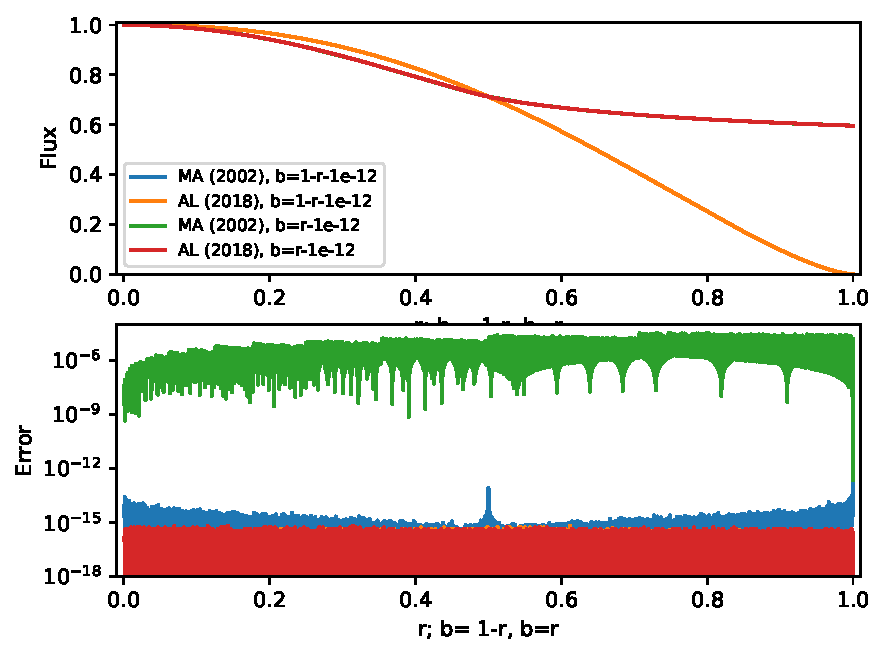
\includegraphics[width=\linewidth]{figures/julia/compare_MA2002_linear.pdf}
    \caption{Comparison of Mandel \& Agol (2002) with Agol \& Luger (2018).}
    \label{fig:compareMA}
    \end{centering} 
\end{figure}

\subsection{Derivative comparison with P\'al}

We have computed the quadratic limb-darkened light curve using the \texttt{F77}
code written by Andr\'as P\'al, \texttt{ntiq\_fortran.f}.  
Figure \ref{fig:Pal_comparison} shows the results of this comparison.
The light curve models agree quite well, as do the derivatives, which is
a good check on both codes.  However, we find that the P\'al model only
achieves single precision for the computation, with errors reaching as
much as a few $\times 10^{-8}$ for the flux and the derivatives with
respect to the limb-darkening parameters.  \citet{Pal2008} uses the
Carlson implementation of elliptic integrals \citep{Carlson1979},
which in practice we find can be both less precise and slower to
evaluate than the \citet{Bulirsch1965a} code for computing elliptic
integrals.

We have also compared the evaluation speed of our code with P\'al's as well.
We compiled P\'al's code using \texttt{gfortrans -O3}, and found that
the computation of quadratic limb-darkened light curves and
derivatives takes an average of 0.52 seconds to compute $10^6$ models, 
while the \texttt{transit\_poly\_struct.jl} takes an average of 0.29 seconds, 
giving our Julia code a 44\% speed advantage over the Fortran code;
we have yet to optimize all aspects of the code, so there may be room
for improvement on this benchmark.

\begin{figure}
    \begin{centering}
    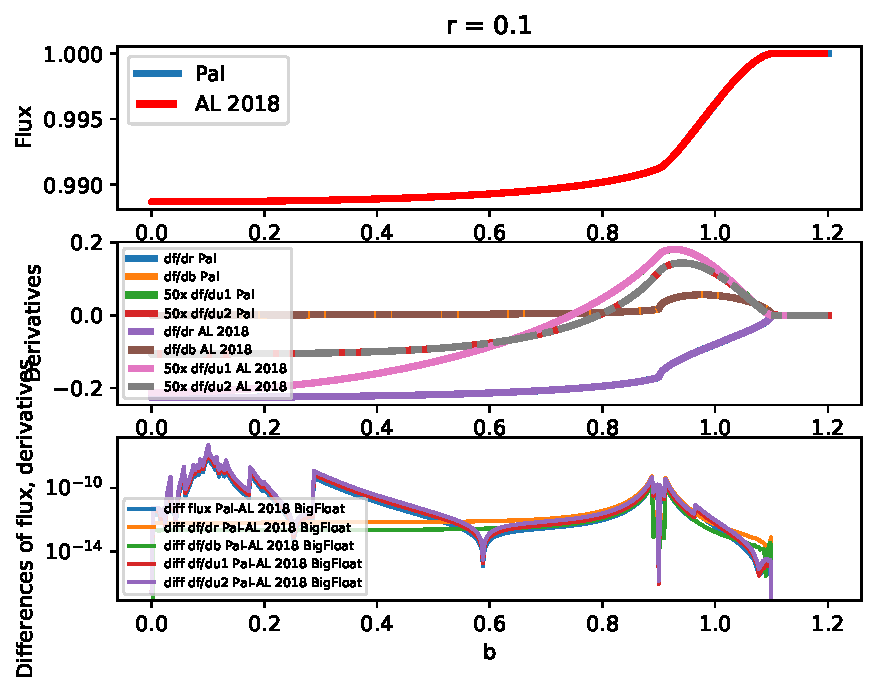
\includegraphics[width=\linewidth]{figures/julia/compare_pal_r0pt1.pdf}
    \caption{Comparison of \citet{Pal2008} with Agol \& Luger (2018).}
    \label{fig:Pal_comparison}
    \end{centering} 
\end{figure}

\begin{itemize}
\item Compare with Gimenez for speed and accuracy for higher order limb-darkening. [ ]
\item Compare with Batman for speed and accuracy. [ ]
\item Compare derivatives with Pal for speed and accuracy. [x]
\item Show the scaling with the number of points in the light curve
and with the number of limb-darkening components. [x]
\end{itemize}

\section{Discussion}

We have presented formulae for the transit (or occultation/eclipse) of a 
limb-darkened body with a limb-darkening profile which is given by a polynomial 
in $\upmu$.  These formulae have multiple assumptions built in:  both bodies 
are treated as spherical \citep{Seager2002,Hui2002}, so that their projected
sufaces are assumed to be circular \citep{Barnes2003,Barnes2004,Barnes2009b};  limb-
darkening is treated as azimuthally-symmetric \citep{Barnes2009a}; refraction 
and any relativistic effects are ignored \citep{Sidis2010}; the edges of both 
bodies are assumed to have a sharp boundary.
All of these assumptions are violated in every transit event to some extent, 
but in many cases can yield an adequate approximation given a particular
signal-to-noise ratio.

However, any model for the surface brightness of a star can only be approximate:  
most stars are convective, rotationally-oblate, spotted, oscillating, flaring, 
etc.  The model we have presented, then, will only resemble any given star to
a precision which is limited by the lack of uniformity of the actual stellar 
surface.  This begs the question of why a numerically precise model is required 
for modelling transit light curves.  The answer is computational accuracy
and stability: this more accurate model can be used over all of parameter space, 
and the high precision enables computation of derivatives which are beneficial 
when optimizing model parameters, computing the Fisher information matrix, or
deriving parameter posteriors with MCMC.

Since we are limited in the knowledge of the properties of any given star, 
the discrepancies of an azimuthally-symmetric limb-darkened model can be 
treated as a source of noise.
The deviation of the star from the model can be absorbed into noise models that 
account for outliers, account for correlations in the noise, or actually
try to model the deviations of the star from azimuthal symmetry 
\citep[e.g.][]{SanchisOjeda2011}.

In additional to the variability and inhomogeneity of stars, the limb-darkening model
can only describe the variation of surface brightness with a limited accuracy.
Our analytic model can be thought of as a Taylor series with which the
limb-darkening can be expanded to as high an order as the data require.
In fact, for planetary transits in which $r$ is small, an arbitrary limb-darkening 
model could be treated as a Taylor series about the location of the planet,
using the analytic formulae to compute an approximate light curve.  This
would require varying the polynomial limb-darkening coefficients as the
planet moved across the disk of the star, which would need to be propagated
through the derivatives properly.  Such a model could be a faster, and
perhaps, more accurate way to treat arbitrary limb-darkening laws, such
as ``non-linear" limb-darkening \citep{Claret2000} or power-law limb-darkening
\citep{Maxted2018}.

One question is what order of the limb-darkening model to choose to
fit the data?  Here we suggest several possibile solutions.  The order of the
limb-darkening can be varied until the chi-square no longer improves (subject
to a penalty for the greater freedom in the model, such as Bayesian Information
Criterion).  A high-order limb-darkening model can be chosen, with the
coefficients regularized to favor small values;  should the data require
a higher-order model, then the coefficients will increase to acommodate
the data.  The parameterization of the limb-darkening with terms with
$d_n ((n+2)\upmu^n-\upmu^{n-2})$ for $n \ge 2$ may be particularly
convenient for this model in that these terms do not contribute to the
total flux of the star.  A third possibility is to fit stellar atmosphere
models with the polynomial limb-darkening model until a sufficient precision
is reached given that warranted by the data, and then to place priors
on the limb-darkening parameters. 

Example applications:  
\begin{enumerate}
\item optimization with and without analytic derivatives;
\item fitting to stellar limb-darkening models;
\item time integrated model with derivatives;
\item HMC.
\end{enumerate}

\section{Conclusions}

We have presented an analytic model for the transits, occultations, and
eclipses of limb-darkened bodies with a polynomial dependence of the limb-darkening
on the $z$ component of the stellar surface (or, alternatively, the
cosine of the angle from the sub-stellar point).  The model is more precise
and accurate than prior models that we have compared to, especially in near 
special limits such as the points of contact and the coincidence of the edge 
of the occultor with the center of the source.  The model also compares favorably in
speed of evaluation, about a factor of two faster than the code due
to \citet{Pal2008}, XXX faster than Gimenez, YYY faster than batman,
and ZZZ faster than ExoFast.

We expect that this code may be used both as a workhorse model for
general fitting of transit models, as well as a tool for more 
specialized applications, such as photodynamical modeling of
interacting planets, triple stars, and transiting circumbinary planets.
{\color{red} Add references for these use cases.}

The code is open source, and has two versions:  one of which is a part
of the \starry package, \texttt{http://github.com/luger/starry/}, written
in a combination of C++ and Python, and a new code written in Julia as
part of the development of the equations in this paper,
\texttt{http://github.com/luger/limbdark/}.

\acknowledgements

We thank Andr\'as P\'al for sharing his Fortran code, \texttt{ntiq-fortran.f}.
We thank Andr\'as P\'al, Kevin Stevenson, Kai Ueltzh\"offer, Mario Damasso,
Matthew Heising, Robert Morehead, and Laura Kreidberg for pointing out
errors or inaccuracies in the Mandel \& Agol paper and code, which we have
hopefully rectified in this paper. 
E.A. acknowledges NSF grant AST-1615315, NASA grant NNX14AK26G and from 
the NASA Astrobiology Institute's Virtual Planetary Laboratory Lead Team, 
funded through the NASA Astrobiology Institute under solicitation NNH12ZDA002C 
and Cooperative Agreement Number NNA13AA93A.

\bibliography{limbdark}

\appendix

Here are a list of errata for \citet{MandelAgol2002}:
\begin{enumerate}
\item In equation 7, $\lambda_3$ and $\lambda_4$ should have $2k \rightarrow
2p$ in arguments of the elliptic integrals.

\item In equation 7, $\lambda_5$ should have $- \frac{2}{3}\Theta(p-1/2)$
at the end.

\item For Case 11 in Table 1, $\eta^d$ should be 1/2, not 1, and
$\lambda^d$ should be zero, not 1.  This mistake affects the code,
but it is never encountered for planets that transit main-sequence
stars since $p<1$.  This typo was discussed in \citet{Eastman2013}.

\item The case $z=1-p$ is missing for $z<p$ (as pointed out by
Pal 2008).

\item There is a $\pi$ missing in the denominator of the second term
on the right hand side of equation (8).
\end{enumerate}

With the exception of 3, none of these errors affected the publicly
available code.
\end{document}
